

\tikzset{every picture/.style={line width=0.75pt}} %set default line width to 0.75pt        

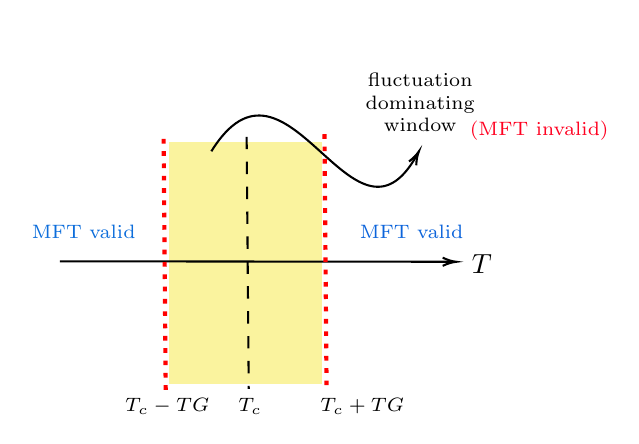
\begin{tikzpicture}[x=0.75pt,y=0.75pt,yscale=-1,xscale=1]
%uncomment if require: \path (0,300); %set diagram left start at 0, and has height of 300

%Shape: Rectangle [id:dp5432386973423167] 
\draw  [draw opacity=0][fill={rgb, 255:red, 248; green, 238; blue, 118 }  ,fill opacity=0.71 ] (152.5,62.49) -- (226.5,62.49) -- (226.5,178.96) -- (152.5,178.96) -- cycle ;
%Straight Lines [id:da864566896446448] 
\draw    (100,120) -- (289,120.21) ;
\draw [shift={(291,120.22)}, rotate = 180.06] [color={rgb, 255:red, 0; green, 0; blue, 0 }  ][line width=0.75]    (6.56,-1.97) .. controls (4.17,-0.84) and (1.99,-0.18) .. (0,0) .. controls (1.99,0.18) and (4.17,0.84) .. (6.56,1.97)   ;
%Straight Lines [id:da4949499900212819] 
\draw  [dash pattern={on 4.5pt off 4.5pt}]  (190,60) -- (191,181.45) ;
%Straight Lines [id:da9090151534187403] 
\draw [color={rgb, 255:red, 255; green, 0; blue, 0 }  ,draw opacity=1 ][line width=1.5]  [dash pattern={on 1.69pt off 2.76pt}]  (150,61) -- (151,182.45) ;
%Straight Lines [id:da17159682825776768] 
\draw [color={rgb, 255:red, 255; green, 0; blue, 0 }  ,draw opacity=1 ][line width=1.5]  [dash pattern={on 1.69pt off 2.76pt}]  (227.5,58.77) -- (228.5,180.22) ;
%Curve Lines [id:da15314304218762675] 
\draw    (173,67) .. controls (209.63,7.93) and (241.36,123.97) .. (272.07,68.73) ;
\draw [shift={(273,67)}, rotate = 117.59] [color={rgb, 255:red, 0; green, 0; blue, 0 }  ][line width=0.75]    (6.56,-1.97) .. controls (4.17,-0.84) and (1.99,-0.18) .. (0,0) .. controls (1.99,0.18) and (4.17,0.84) .. (6.56,1.97)   ;

% Text Node
\draw (224,184.4) node [anchor=north west][inner sep=0.75pt]  [font=\scriptsize]  {$T_{c} +T\tund{G}$};
% Text Node
\draw (184.5,184.4) node [anchor=north west][inner sep=0.75pt]  [font=\scriptsize]  {$T_{c}$};
% Text Node
\draw (297,115.4) node [anchor=north west][inner sep=0.75pt]    {$T$};
% Text Node
\draw (224,28) node [anchor=north west][inner sep=0.75pt]  [font=\scriptsize] [align=left] {\begin{minipage}[lt]{72.14pt}\setlength\topsep{0pt}
\begin{center}
fluctuation dominating\\window
\end{center}

\end{minipage}};
% Text Node
\draw (85,100.8) node [anchor=north west][inner sep=0.75pt]  [font=\scriptsize,color={rgb, 255:red, 12; green, 109; blue, 219 }  ,opacity=1 ] [align=left] {MFT valid};
% Text Node
\draw (243,100.8) node [anchor=north west][inner sep=0.75pt]  [font=\scriptsize,color={rgb, 255:red, 12; green, 100; blue, 219 }  ,opacity=1 ] [align=left] {MFT valid};
% Text Node
\draw (296,50.8) node [anchor=north west][inner sep=0.75pt]  [font=\scriptsize,color={rgb, 255:red, 255; green, 0; blue, 32 }  ,opacity=1 ] [align=left] {(MFT invalid)};
% Text Node
\draw (130,184.4) node [anchor=north west][inner sep=0.75pt]  [font=\scriptsize]  {$T_{c} - T\tund{G}$};


\end{tikzpicture}
